\chapter{Factor analysis}
\label{factanal}

\section{Role of factor analysis}
\label{rolefa}

Most of the development of factor analysis has taken place outside the statistical community, most often in terms of Psychometrics which may partly reflect its origins in the study of intelligence.   The earliest cited reference is \cite{Spearman:1904}.  Factor Analysis and Principal Components Analysis are often confused with each other, just to be really awkward there is one method of performing Factor Analysis called Principal Component Extraction.   The two methods should never be confused.   Principal Components seeks orthogonal projections of the data according the variance maximisation with the hope of achieving some dimension reduction.   Factor analysis is all about studying the co-variance (or correlation) and is based on a statistical model.  We hope to describe the covariance relationships between many variables in terms of a few underlying, unobservable random quantities called factors.   If there is a group of highly correlated variables, which in turn are uncorrelated with other variables, perhaps these represent realisations of some underlying phenomena that is responsible for for the observed correlations.   It is an attempt to approximate the covarariance matrix $\boldsymbol{\Sigma}$.  It is not highly regarded by many statisticians, but it is used by many others.   There are currently many variations on a theme (such as Structural Equation Modelling) which are also very common in many applied literatures.



Whilst we can consider one model for factor analysis, there are two very different fitting methods, neither of which is entirely satisfactory.   Having found a solution there are a large number of possible rotations of the solution each of which aim to give the most interpretable solution.   In other words, don't be surprised if different computer programs give different ``Factor Analysis'' solutions for the same data.


\begin{figure}
\begin{picture}(100,200)(0,0)

\put(0,150){\fbox{f1}}
\put(30,150){\vector(2,-1){95}} 
\put(30,150){\vector(2,1){95}} 
\put(30,150){\vector(1,-1){95}} 

\put(0,50){\fbox{f2}}
\put(30,50){\vector(2,-1){95}} 
\put(30,50){\vector(2,1){95}} 
\put(30,50){\vector(1,1){95}}  

\put(150,0){\fbox{X1}}
\put(150,100){\fbox{X2}}
\put(150,200){\fbox{X3}}

\end{picture}
\caption{Factor analysis, dependence between three variables represented by two latent variables - is this sensible}
\end{figure}

Factor Analysis is normally carried out with a view to reification: the investigator usually has a conceptual model of some underlying entity which cannot be measured directly.   These latent, or hidden, variables are the factors in factor analysis.   The aim of factor analysis is that each of the $p$ observed variables can be represented by means of $q<p$ mutually uncorrelated common factors.   This will leave some uncorrelated residual specific to each of the observed variables, the uniqueness, which is not correlated with any of the remaining $p-1$ variables \footnote{Note that the diagonal of a correlation matrix is 1. This statement implies that only part of this 1 is due to the $q<p$ latent variables - this part is known as the communality.}.   It is possible to rotate the $q$ axes of common factors to new orthogonal or obligue axes to make the factor solution fit with existing theoretical ideas regarding the model.  

\section{The factor analysis model}
\label{factanalmodel}

The orthogonal model underlying Factor Analysis can be described as follows:

\begin{displaymath}
\label{factanal}
\boldsymbol{x} = \boldsymbol{\mu} + \boldsymbol{\Gamma} \boldsymbol{\phi} + \boldsymbol{\zeta}
\end{displaymath}

Where $\boldsymbol{x}$ is an $1 \times p$ random vector.   $\boldsymbol{\mu}$ represents a vector of unknown constants (mean values), $\boldsymbol{\Gamma}$ is an unknown $p \times q$ matrix of constants referred to as the \textit{loadings}.   $\boldsymbol{\phi}$ is a $q \times 1$ unobserved random vector referred to as the \textit{scores} assumed to have mean $\boldsymbol{0}$ and covariance $\boldsymbol{\Sigma}_{\phi}$, it is commonly assumed that $\boldsymbol{\Sigma}_{\phi} = \boldsymbol{I}$.   $\boldsymbol{\zeta}$ is $1 \times p$ unobserved random error vector having mean $\boldsymbol{0}$ and by assumption a diagonal covariance $\boldsymbol{\psi}$ referred to as the \textit{uniqueness} or \textit{specific variance}.   

With these assumptions, $cov(\boldsymbol{\phi}, \boldsymbol{\zeta}) = 0$, if $\boldsymbol{\Sigma}_{\phi} = \boldsymbol{I}$ then $cov(\boldsymbol{x}, \boldsymbol{\phi}) = \boldsymbol{\Gamma}$.   It is worth emphasising that unlike many multivariate techniques covered here, factor analysis is a statistical model for our observations, with the following distributional form:

\begin{displaymath}
\boldsymbol{x} \sim Normal(\boldsymbol{\mu}, \boldsymbol{\Gamma} \boldsymbol{\Gamma}^{T} + \boldsymbol{\psi})
\end{displaymath}

It may be slightly clearer to consider the way a vector of observations $\boldsymbol{x} = x_{1}, \ldots, x_{p}$ are modelled in factor analysis:

\begin{eqnarray*}
x_{1} &=& \mu_{1} + \sum_{k=1}^{q} \gamma_{1k} \phi_{k}  + \zeta_{1}\\
x_{2} &=& \mu_{2} + \sum_{k=1}^{q} \gamma_{2k} \phi_{k}  + \zeta_{2}\\
&\vdots&\\
x_{p} &=& \mu_{p} + \sum_{k=1}^{q} \gamma_{pk} \phi_{k}  + \zeta_{p}
\end{eqnarray*}

Note that under the terms of this model:

\begin{equation}
\label{communalities}
var(x_{j}) = \gamma_{j1}^{2} + \gamma_{j2}^{2} + \ldots + \gamma_{jq}^{2} + var(\zeta_{j})
\end{equation} 

One potential problem with this model should be immediately obvious, there can be rather more parameters than data.   For example, note that the covariance matrix $\boldsymbol{\Sigma}$ has $p(p+1)/2$ parameters, the factor model $ \boldsymbol{\Gamma} \boldsymbol{\Gamma}^{T} + \boldsymbol{\psi})$ has $qp - q(q-1)/2 + p$ parameters.  One issue arises whereby a factor analsis model must be constrained in order to ensure identifiability.  Clearly, $p(p+1)/2 \geq qp - q(q-1)/2 + p$, or:

\begin{equation}
\label{qp}
q \leq \frac{2p + 1 - \sqrt{8p-1}}{2}
\end{equation}

This gives some maximum values of $q$ for given values of $p$:


\begin{tabular}{rr}
\hline
$p$ & max $q$ \\
\hline
1 & 0\\
2 & 0\\ 
3 & 1\\
4 & 1\\
5 & 2\\
6 & 3\\
7 & 3\\
8 & 4\\
9 & 5\\
10 & 6\\
\hline
\end{tabular}

Where $q<p$, the right hand side of \ref{communalities} indicates how much of $var(x_{j}$ is explained by the model, a concept referred to as the communality.   Consideration of the order of the model leads on to a point we will consider later, degrees of freedom after fitting a $q$ factor model:

\begin{equation}
\label{dffact}
df = \frac{p(p+1)}{2} - qp + \frac{q(q-1)}{2} - p = \frac{(p-q)^{2} - (d+m)}{2}
\end{equation}


\subsection{Centred and standardised data}

In practice it is often much simpler to centre the data, so that we model:

\begin{equation}
\label{facentre}
x_{j} - \mu_{j} = \sum_{k=1}^{q} \gamma_{k} \phi_{k} + \zeta_{j}; j = 1, \ldots, p
\end{equation}

or even to standardise the variables so that in effect we are modelling the correlation matrix rather than the covariance matrix.   

\begin{equation}
\label{fastandardise}
\frac{x_{j} - \mu_{j}}{\sigma_{jj}} = \sum_{k=1}^{q} \gamma_{k} \phi_{k} + \zeta_{j}; j = 1, \ldots, p
\end{equation}


Regardless of the data matrix used, factor analysis is essentially a model for $\boldsymbol{\Sigma}$, the covariance matrix of $\boldsymbol{x}$, 

\begin{displaymath}
\label{covdecomp}
\boldsymbol{\Sigma} = \boldsymbol{\Gamma}\boldsymbol{\Gamma}^{T} + \boldsymbol{\psi}
\end{displaymath}

\subsection{Factor indeterminacy}

We now consider another problem with factor analysis.   It is a very indeterminate model, specifically it is unchanged if we replace $\boldsymbol{\Gamma}$ by $\boldsymbol{K} \boldsymbol{\Gamma}$ for any orthogonal matrix $\boldsymbol{K}$.   However, this can be turned to our advantage, with sensible choice of a suitable orthogonal matrix $\boldsymbol{K}$ we can achieve a rotation that may yield a more interpretable answer.  Factor analysis therefore requires an additional stage, having fitted the model we may wish to consider rotation of the coefficients.  

\subsection{Strategy for factor analysis}

 To fit the model, we therefore need to:

\begin{itemize}
\item Estimate the number of common factors $q$.   
\item Estimate the factor loadings $\boldsymbol{\Gamma}$
\item Estimate the specific variances $\boldsymbol{\psi}^{2}$
\item On occasion, estimate the factor scores $\boldsymbol{\phi}$
\end{itemize}


We will now consider fitting methods for factor analysis.   It will be obvious that the preferred method in R is the maximum likelihood method, but we will first consider methods based around principal components to reinforce some ideas about the model.

\section{Principal component extraction}

We have already used the spectral decomposition to obtain one possible factoring of the covariance matrix $\boldsymbol{\Sigma}$.

\begin{displaymath}
\boldsymbol{\Sigma} = \boldsymbol{E} \boldsymbol{\Lambda}\boldsymbol{E}^{T}
\end{displaymath}

which can be expanded:

\begin{eqnarray*}
\boldsymbol{\Sigma} &=& \lambda_{1} \boldsymbol{e}_{1} \boldsymbol{e}_{1}^{T} +  \lambda_{2} \boldsymbol{e}_{2} \boldsymbol{e}_{2}^{T} + \ldots  \lambda_{p} \boldsymbol{e}_{p} \boldsymbol{e}_{p}^{T} \\
 &=& \left( \sqrt{\lambda_{1}} \boldsymbol{e}_{1}, \sqrt{\lambda_{2}} \boldsymbol{e}_{2}, \ldots, \sqrt{\lambda_{p}} \boldsymbol{e}_{p} \right) \left( \begin{array}{c} \sqrt{\lambda_{1}} \boldsymbol{e}_{1} \\  \sqrt{\lambda_{2}} \boldsymbol{e}_{2} \\ \vdots \\  \sqrt{\lambda_{p}} \boldsymbol{e}_{p} \end{array} \right)
\end{eqnarray*}

Of course, in practice we don't know $\boldsymbol{\Sigma}$ and we use  $S$ (or we standardise the variables and use $R$ - it should be remembered that this is rather a big decision when working with principal components).   Referring back to our data, it should be remembered that the spectral decomposition yields linear principal components as follows:

\begin{eqnarray*}
z_{1} &=& e_{11}x_{1} + e_{12}x_{2} + \ldots + e_{1p} x_{p}; var(z_{1})=\lambda_{1}\\
z_{2} &=& e_{21}x_{2} + e_{22}x_{2} + \ldots + e_{2p} x_{p}; var(z_{2})=\lambda_{2}\\
&\vdots&\\
z_{p} &=& e_{p1}x_{1} + e_{p2}x_{1} + \ldots + e_{1p} x_{p}; var(z_{p})=\lambda_{p}
\end{eqnarray*}

which in matrix notation this can be expressed as: 

\begin{equation}
\label{pcfact}
\boldsymbol{Z} = \boldsymbol{E}\boldsymbol{X}
\end{equation}

where  $\boldsymbol{Z} = \left( \begin{array}{c} z_{1} \\ z_{2} \\ \vdots \\ z_{p} \end{array} \right)$,  $\boldsymbol{X} = \left( \begin{array}{c} X_{1} \\ X_{2} \\ \vdots \\ X_{p} \end{array} \right)$ and  $\boldsymbol{E} = \left( \begin{array}{cccc} e_{11} & e_{12} & \hdots & e_{1p} \\ 
e_{21}& e_{22} & \hdots & e_{2p} \\
 \vdots & \vdots & \ddots & \vdots \\ 
e_{p1} & e_{p2} & \hdots & e_{pp}  \end{array} \right)$.   

Multiplying both sides of \ref{pcfact} by $\boldsymbol{E}^{-1}$gives:

\begin{equation}
\boldsymbol{E}^{-1} \boldsymbol{Z} = \boldsymbol{X}
\end{equation}

We know orthogonal matrices generally that $\boldsymbol{E}^{-1} = \boldsymbol{E}^{T}$ so we can invert the transformation by using

\begin{equation}
\boldsymbol{X} = \boldsymbol{E}^{T} \boldsymbol{Z}
\end{equation}

which can be expanded as:

\begin{eqnarray*}
x_{1} &=& e_{11}z_{1} + e_{21} z_{2}  + \ldots + e_{p} z_{p}  \\
x_{2} &=& e_{12}z_{2} + e_{22} z_{2} + \ldots + e_{p} z_{p}  \\
&\vdots& \\
x_{p} &=& e_{1p}z_{1} + e_{2p} z_{2} + \ldots + e_{pp} z_{p}  
\end{eqnarray*}

which we could express as;

\begin{eqnarray*}
x_{1} &=& (e_{11} \sqrt{\lambda_{1}}) \frac{z_{1}}{\sqrt{\lambda_{1}}} + (e_{21} \sqrt{\lambda_{2}}) \frac{z_{2}}{\sqrt{\lambda_{2}}} + \ldots +  (e_{p1} \sqrt{\lambda_{p}}) \frac{z_{p}}{\sqrt{\lambda_{p}}} \\
x_{2} &=& (e_{12} \sqrt{\lambda_{1}}) \frac{z_{1}}{\sqrt{\lambda_{1}}} + (e_{12} \sqrt{\lambda_{1}}) \frac{z_{1}}{\sqrt{\lambda_{1}}} + \ldots +  (e_{p2} \sqrt{\lambda_{p}}) \frac{z_{p}}{\sqrt{\lambda_{p}}} \\
&\vdots& \\
x_{p} &=& (e_{1p} \sqrt{\lambda_{1}}) \frac{z_{1}}{\sqrt{\lambda_{1}}} + (e_{2p} \sqrt{\lambda_{2}}) \frac{z_{2}}{\sqrt{\lambda_{2}}} + \ldots +  (e_{pp} \sqrt{\lambda_{p}}) \frac{z_{p}}{\sqrt{\lambda_{p}}} 
\end{eqnarray*}

and if we set $\gamma_{jk} = (e_{jk} \sqrt{\lambda_{j}})$ and $\phi_{j} = z_{j} / \sqrt{\lambda_{j}}$ we have a clear link with the factor analysis model given in equation \ref{factanal}.   If we try writing this in matrix terminology, our loadings matrix $\boldsymbol{\Gamma}$ is the $p \times p$ matrix where the $j$th column is given by  $\sqrt{\lambda_{j}} \boldsymbol{e}_{j}$ we now have:

\begin{displaymath}
\boldsymbol{S} = \boldsymbol{\Gamma} \boldsymbol{\Gamma}^{T}
\end{displaymath}

which is getting us part of the way to our factor analysis model.   Before going any further we will reinforce this procedure by considering how to obtain these values from within R.  Note that under the principal component solution, the estimated loadings do not alter as the number of factors is increased or decreased. We are going to load the economic data, and carry out a decomposition of the correlation matrix $\boldsymbol{R}$.

\singlespacing
\begin{verbatim}
> econ <- read.csv("econ.csv", row.names = 1)
> econ.cor <- cor(econ)
> econ.ev <- eigen(econ.cor)
> loadings <- matrix(0,9,9)
> for (i in 1:9){
> loadings[,i] <- sqrt(econ.ev$values[i]) * econ.ev$vectors[,i]
> }
> econ.cor - loadings %*% t(loadings) ## should equal zero
\end{verbatim}
\onehalfspacing



Clearly we don't actually want to use a decomposition with with $q=p$ variables.   As might be rather obvious bearing in mind our earlier use of principal components, we wish to partition $\boldsymbol{\Lambda}$ into $\boldsymbol{\Lambda}_{1} = \lambda_{1}, \lambda_{2}, \ldots, \lambda_{q}$ and $\boldsymbol{\Lambda_{2}} = \lambda_{q+1}, \ldots, \lambda_{p}$ with the corresponding eigenvectors.   As a consequence, we reduce the size of our $\boldsymbol{\Gamma}$ matrix, i.e. to neglect the contribution of  $\lambda_{q+1} \boldsymbol{e}_{q+1} \boldsymbol{e}_{q+1}^{T} + \ldots  \lambda_{p} \boldsymbol{e}_{p} \boldsymbol{e}_{p}^{T}$.   So when considering our model for the data, we wish to partition our factors as follows:

\begin{eqnarray*}
x_{1} &=& e_{11}z_{1} + e_{21} z_{2}  + \ldots + e_{q1} z_{q} +  e_{q+1,1} z_{q+1} + \ldots +  e_{p1} z_{p} \\
x_{2} &=& e_{12}z_{2} + e_{22} z_{2} + \ldots + e_{q2} z_{q} +  e_{q+1,2} z_{q+1} + \ldots + e_{p2} z_{p} \\
&\vdots& \\
x_{p} &=& e_{1p}z_{1} + e_{2p} z_{2} + \ldots + e_{qp} z_{q} + e_{q+1,p} z_{q+1} + \ldots + e_{pp} z_{p} 
\end{eqnarray*}

and if we set $ e_{q+1,j} z_{q+1} + \ldots +  e_{pj} z_{p} = \zeta_{j}; j = 1, \ldots, p$ we can rewrite this as:


\begin{eqnarray*}
x_{1} &=& e_{11} z_{1} + e_{21} z_{2} + \ldots + e_{q1} z_{q} +  \zeta_{1}\\
x_{2} &=& e_{12} z_{1} + e_{22} z_{2} + \ldots + e_{q2} z_{q} +  \zeta_{2}\\
&\vdots& \\
x_{p} &=& e_{1p} z_{1} + e_{2p} z_{1} + \ldots + e_{qp} z_{q} + \zeta_{p}
\end{eqnarray*}

As earlier, we can expressed this as:

\begin{eqnarray*}
x_{1} &=& (e_{11} \sqrt{\lambda_{1}}) \frac{z_{1}}{\sqrt{\lambda_{1}}} + (e_{21} \sqrt{\lambda_{2}}) \frac{z_{2}}{\sqrt{\lambda_{2}}} + \ldots +  (e_{q1} \sqrt{\lambda_{q}}) \frac{z_{q}}{\sqrt{\lambda_{q}}} +  \zeta_{1}\\
x_{2} &=& (e_{12} \sqrt{\lambda_{1}}) \frac{z_{1}}{\sqrt{\lambda_{1}}} + (e_{12} \sqrt{\lambda_{1}}) \frac{z_{1}}{\sqrt{\lambda_{1}}} + \ldots +  (e_{q2} \sqrt{\lambda_{q}}) \frac{z_{q}}{\sqrt{\lambda_{q}}} +  \zeta_{2}\\
&\vdots& \\
x_{p} &=& (e_{1p} \sqrt{\lambda_{1}}) \frac{z_{1}}{\sqrt{\lambda_{1}}} + (e_{2p} \sqrt{\lambda_{2}}) \frac{z_{2}}{\sqrt{\lambda_{2}}} + \ldots +  (e_{qp} \sqrt{\lambda_{q}}) \frac{z_{q}}{\sqrt{\lambda_{q}}} +  \zeta_{p}
\end{eqnarray*}

where $\gamma_{jk} = (e_{jk} \sqrt{\lambda_{j}})$ and $\phi_{i} = z_{i} / \sqrt{\lambda_{i}}$ as before, notice as stated at the outset that $var(\boldsymbol{\zeta}) = \boldsymbol{\psi}$.   If we consider this in terms of the decomposition of the covariance matrix we have:

\begin{equation}
\boldsymbol{\Sigma} = \left( \sqrt{\lambda_{1}} \boldsymbol{e}_{1}, \sqrt{\lambda_{2}} \boldsymbol{e}_{2}, \ldots, \sqrt{\lambda_{q}} \boldsymbol{e}_{q} \right) \left( \begin{array}{r} \sqrt{\lambda_{1}} \boldsymbol{e}_{1} \\  \sqrt{\lambda_{2}} \boldsymbol{e}_{2} \\ \vdots \\  \sqrt{\lambda_{q}} \boldsymbol{e}_{q} \end{array} \right) + 
\left[ \begin{array}{rrrr} \psi_{1} & 0 & \hdots & 0\\
0 & \psi_{2} & \hdots & 0\\
\vdots & \vdots & \ddots & \vdots\\
0 & 0 & \hdots & \psi_{p}
\end{array} \right]
\end{equation}

Where now $\psi_{j} = var(\zeta_{j}) =  \sigma_{jj} - \sum_{k=1}^{q} \gamma_{jk}^{2}$ for $k = 1, 2, \ldots, q$. 

Estimates of the specific variances are given by diagonal elements of the matrix $\boldsymbol{\hat{\Sigma}} - \boldsymbol{\hat{\Gamma}}\boldsymbol{\hat{\Gamma}}^{T}$, i.e:

\begin{equation}
\boldsymbol{\hat{\psi}} = 
\left[ \begin{array}{rrrr} \psi_{1} & 0 & \hdots & 0\\
0 & \psi_{2} & \hdots & 0\\
\vdots & \vdots & \ddots & \vdots\\
0 & 0 & \hdots & \psi_{p}
\end{array} \right]
\mbox{with}  \psi_{j} = \sigma_{jj} - \sum_{k=1}^{q} \gamma_{jk}^{2}
\end{equation}



So, when using the principal component solution of $\boldsymbol{\hat{\Sigma}}$, it is specified in terms of eigenvalue-eigenvector pairs ($\hat{\lambda}_{1}, \hat{\boldsymbol{e}}_{1}$), ($\hat{\lambda}_{2}, \hat{\boldsymbol{e}}_{2}$), $\ldots$, ($\hat{\lambda}_{p}, \hat{\boldsymbol{e}}_{p}$), where $\hat{\lambda}_{1} \geq \hat{\lambda}_{2} \geq \ldots \geq \hat{\lambda}_{p}$.   If we wish to find a $q<p$ solution of common factors, then the estimated factor loadings are given by:

\begin{displaymath}
\boldsymbol{\hat{\Gamma}} = \left( \sqrt{\lambda_{1}} \boldsymbol{e}_{1}, \sqrt{\lambda_{2}} \boldsymbol{e}_{2}, \ldots, \sqrt{\lambda_{q}} \boldsymbol{e}_{q} \right) 
\end{displaymath}

As with the factor analysis model given earlier, the factors $\boldsymbol{\phi}$ have identity covariance matrix

\begin{displaymath}
var(\boldsymbol{\phi}) = var \left(\sqrt{\Lambda_{1}} \boldsymbol{\Gamma}_{1}^{T}(\boldsymbol{x} - \boldsymbol{\mu}) \right) = \boldsymbol{I}_{q},
\end{displaymath}

 and are uncorrelated with the residuals:

\begin{displaymath}
cov(\boldsymbol{\phi}, \boldsymbol{\zeta}) = cov \left( \sqrt{\Lambda_{1}} \boldsymbol{\Gamma}_{1}^{T}(\boldsymbol{x} - \boldsymbol{\mu}),  \boldsymbol{\Gamma}_{2}\boldsymbol{\Gamma}_{2}^{T}(\boldsymbol{x} - \boldsymbol{\mu}) \right) = \sqrt{\boldsymbol{\Lambda_{1}}} \boldsymbol{\Gamma}_{1}^{T} \boldsymbol{\Sigma} \boldsymbol{\Gamma}_{2} \boldsymbol{\Gamma}_{2}^{T} = 0
\end{displaymath}

However, one major objection to this principal component ``solution'' is that it can also be seen that each $\zeta_{i}$ contains the same $z_{i}$ so they are not mutually unrelated.   Hence the latent variables obtained using the principal component method do not explain all the correlation structure in our data $\boldsymbol{X}$.   The covariance matrix for the errors is now:

\begin{displaymath}
var(\boldsymbol{\zeta}) = \boldsymbol{\Gamma}_{2} \boldsymbol{\Lambda}_{2} \boldsymbol{\Gamma}_{2}^{T}
\end{displaymath}


This additional step can be carried out fairly easily in R.   We only need to discard the unwanted components and estimate the uniquenesses:

\singlespacing
\begin{verbatim}
> loadings4 <- matrix(0,9,4)
> for (i in 1:4){
> loadings4[,i] <- sqrt(econ.ev$values[i]) * econ.ev$vectors[,i]
> }
> LLt <- loadings4 %*% t(loadings4)
> unique <- diag(econ.cor - LLt)
> error <- econ.cor - (LLt + unique)
\end{verbatim}
\onehalfspacing

and so \texttt{loadings4} gives us the matrix of loadings, \texttt{unique} gives us an estimate of the uniquenesses.  It should be noted that the loadings are unaltered as the number of factors $q$ is changed.   It may be noted that the diagonal elements of $\boldsymbol{\hat{\Sigma}}$ are given by the diagonal elements of $\boldsymbol{\Gamma}\boldsymbol{\Gamma}^{T} + \boldsymbol{\psi}$, but this is not true of the off-diagonal elements.  There are error terms associated with our decomposition of the covariance matrix, these can be easily found from \texttt{error}.  Clearly these are values we wish to see minimised. 

We will consider interpretation of factor structure in more detail later.   However, for now it may be of interest to examine the four factor solution.   It would appear that the first factor represents some kind of contrast between agriculture and other industries (with the exception of finance and mining).

\singlespacing
\begin{verbatim}
\loadings4
                                   [,1]        [,2]        [,3]        [,4]
Agriculture                -0.978199871 -0.07760625  0.05173168 -0.02899271
Mining                     -0.002342834 -0.90214224 -0.21179672 -0.06592893
Manufacture                 0.645370678 -0.52159027 -0.15703856  0.34982446
PowerSupplies               0.476333161 -0.37897538 -0.58769654 -0.39731951
Construction                0.608061420 -0.07694001  0.15838634  0.66387307
ServiceIndustries           0.707975893  0.51045159 -0.12126845  0.05137022
Finance                     0.138717720  0.66237521 -0.61559512  0.05147600
SocialAndPersonalServices   0.723602099  0.32374238  0.32749903 -0.40851903
TransportAndCommunications  0.684640120 -0.29451591  0.39342807 -0.31637790
\end{verbatim}
\onehalfspacing

\subsection{Diagnostics for the factor model}

We can define a residual matrix as:

\begin{equation}
\boldsymbol{\epsilon} = \boldsymbol{{S}} - \left(\boldsymbol{L}\boldsymbol{L}^{T} + \boldsymbol{\psi} \right)
\end{equation}

By construction, the diagonal elements of this residual matrix will be zero.   A decision to retain a particular $q$ factor model could be made depending on the size of the off-diagonal elements.   Rather conveniently, there is an inequality which gives us:

\begin{equation}
\left[ \boldsymbol{\epsilon} = \boldsymbol{\hat{\Sigma}} - \left(\boldsymbol{L}\boldsymbol{L}^{T} + \boldsymbol{\psi} \right) \right] \leq \hat{\lambda}_{q+1}^{2} + \cdots + \hat{\lambda}_{p}^{2}
\end{equation}

So it is possible to check the acceptability of fit in terms of a small sum of squares of neglected eigenvalues.

In a similar manner to that used in principal components, it is possible to use the eigenvalues to indicate the proportion of variance explained by any given factor.   So instead of examining discarded components we could examine those we intend to retain.   Bearing in mind that $trace(\boldsymbol{\Sigma} = \sigma_{11} + \sigma_{22} + \ldots + \sigma_{pp}$, we know that the amount of variation explained by the first factor $\gamma_{11}^{2} + \gamma_{21}^{2} + \ldots + \gamma_{p1}^{2} = (\sqrt{\lambda_{1}} \boldsymbol{e}_{1})^{T}(\sqrt{\lambda_{1}} \boldsymbol{e}_{1}) = \lambda^{1}$.

So we know that the $j$-th factor explains the following proportion of total sample variance:

\begin{equation}
\frac{\lambda_{j}}{trace(\boldsymbol{S})}
\end{equation}

which reduces to $\frac{\lambda_{j}}{p}$ when using standardised variables (the correlation matrix).

It is actually in the context of factor analysis that the Kaiser criterion was developed.   This is implemented by default in a number of computer programs, basically we retain factors which are explaining more than the average amount of variance; if we are decomposing the correlation matrix we retain all factors where the corresponding eigenvalues are greater than one.   We can consider the number of components to retain from our earlier eigen analysis.   The following R output gives the eigenvalues, and the proportion and cumulating proportion explained by each possible factor.

\singlespacing
\begin{verbatim}
> econ.ev$values
[1]  3.482820 2.132332 1.098373 0.9984261 0.5450933
[6] 0.3836385 0.2224905 0.1367327 0.0000930
 
> econ.ev$values / 0.09
[1] 38.698003578 23.692581759 12.204146983 11.093622860  6.056592340
[6]  4.262650255  2.472116648  1.519252072  0.001033506

> cumsum(econ.ev$values/0.09)
[1]  38.69800  62.39059  74.59473  85.68836  91.74495  96.00760  98.47971
[8]  99.99897 100.00000
\end{verbatim}
\onehalfspacing

Considering the eigenvalues first, using the Kaiser criterion would lead us to select three components, but it should be noted that the fourth component is only just below 1 (0.998) giving perhaps some warning as to the arbitrariness of this device.   There are 9 variables, so we divide by 9 (and multiply by 100 to express the proportions as a percentage).   Cumulative values are also given.   We require five components to explain over 90\% of the variation.   Remember that according to formula \ref{qp} this is the largest value of $q$ that can be contemplated with nine manifest variables.


\subsection{Communalities}

Another important concept are the communalities.   In the case of standardised variables, these indicate the proportion of variance of a manifest variable explained by its relevant factor structure.   These are simply estimated as:

\begin{equation}
\xi_{jk}^{2} = \gamma_{j1}^{2} +  \gamma_{j2}^{2} + \cdots +  \gamma_{jq}^{2}
\end{equation}

Terminology can now be supplied for the decomposition of the variance of $\boldsymbol{x}$ given earlier in \ref{communalities} to reflect the reduced dimensionality.   

\begin{equation}
\label{communality}
var(x_{j}) = \underbrace{\gamma_{j1}^{2} + \gamma_{j2}^{2} + \ldots + \gamma_{jq}^{2}}_{communality\ of\ x_{j}} + \underbrace{\psi_{i}}_{specificity\ of\ x_{j}}
\end{equation} 

For standardised variables, $var(x_{j}) = 1$, therefore: $\gamma_{i1}^{2} + \gamma_{i2}^{2} + \ldots + \gamma_{i1}^{q} \leq 1$ and $-1 \leq \gamma_{jk} \leq 1$.

These are fairly simply extracted from our matrix of loadings by squaring all entries and summing by row:

\singlespacing
\begin{verbatim}
> row.names(loadings4) <- row.names(econ.cor)
> apply(loadings4^2, 1, sum)
               Agriculture                     Mining 
                 0.9664145                  0.8630706 
               Manufacture              PowerSupplies 
                 0.8355980                  0.8737656 
              Construction          ServiceIndustries 
                 0.8414721                  0.7791356 
                   Finance  SocialAndPersonalServices 
                 0.8395906                  0.9025525 
TransportAndCommunications 
                 0.8103523 
\end{verbatim}
\onehalfspacing


These appear to be reasonably high for most variables which would suggest a plausible fit for the factor model.


\subsection{Principal Factor solution}

We might have been worried about the way our model above doesn little to account for the off-diagonal elements of $\boldsymbol{\hat{\Sigma}}$.   Principal factoring (which seems to have rather fewer advocates) considering decomposing a reduced matrix.   We know that the diagonal elements of our covariance matrix are given by $\sigma_{jj} = \xi_{j}^{2} + \psi_{j}$, so having determined the number $q$ of common factors needed, we can decompose the reduced covariance matrix.   If we obtain some initial estimates of $\boldsymbol{\psi}$, we can re-estimate the remaining part of the decomposition $\boldsymbol{\Gamma} \boldsymbol{\Gamma}^{T}$.

\begin{equation}
\sigma_{jj} = \xi_{j}^{2} + \psi_{j}
\end{equation}

If we had some initial estimate of $\boldsymbol{\psi}$, $\widetilde{\boldsymbol{\psi}}$ say,  we could obtained a ``reduced'' covariance matrix

\begin{displaymath}
\boldsymbol{S} = \left( \begin{array}{rrrr}
\widetilde{\xi}_{1}^{2} & s_{12} & \cdots & s_{1p}\\
s_{21} & \widetilde{\xi}_{2}^{2} & \cdots & s_{2p}\\
\vdots & \vdots & \ddots & \vdots \\
s_{p1} & s_{p2} & \cdots & \widetilde{\xi}_{p}^{2}
\end{array} \right) 
\end{displaymath}
and carry out an eigendecomposition of this matrix, updating our estimates of the uniqueness and repeat until convergence.

So all we need is an initial estimate of $\widetilde{\boldsymbol{\psi}}$.   Many programs conduct a multiple regression of each manifest variable on each other, and use $s_{jj} r_{j}^{2}$.   We then conduct a principal component analysis on $\boldsymbol{S} - \boldsymbol{\psi}$to find $\boldsymbol{\Gamma}$.   $\boldsymbol{\psi}$ can then be recalculated as the diagonal of $\boldsymbol{S} - \boldsymbol{\Gamma} \boldsymbol{\Gamma}^{T}$ and we extract a further set of principal components.   These latter steps are repeated until convergence, which can be slow if it happens at all.   As we are working with the correlation matrix, it's easy enough to find these intial values:

\singlespacing
\begin{verbatim}
> r2s <- vector("numeric", 9)
> 
> for (i in 1:9){
+ y <- econ[,i]
+ x <- econ[,-i]
+ mod <- lm(y~as.matrix(x))
+ r2s[i] <- summary(mod)$r.squared
+ }
> 
> 
> unique <- diag(1-r2s)
> diag(unique)
[1] 0.0001429627 0.0420230140 0.0006887118 0.1325518542 0.0138610514
[6] 0.0016432160 0.0043879128 0.0007569780 0.0161276459
\end{verbatim}
\onehalfspacing

And all that is now required is to repeatedly implement the loop stage.   This is presented as a function in \texttt{mvmmisc.R}, but it is worth pasting through this manually to see how the procedure works.   

\singlespacing
\begin{verbatim}
> new <- econ.cor - unique
> new.ev <- eigen(new)
> 
> loadings4pf <- matrix(0,9,4)
> for (i in 1:4){
+ loadings4pf[,i] <- sqrt(new.ev$values[i]) * new.ev$vectors[,i]
+ }
> 
> LLt <- loadings4pf %*% t(loadings4pf)
> 
> unique.f <- econ.cor - LLt
> diag(unique) <- diag(unique.f)
> 
> diag(unique)
[1] 0.02890147 0.14965321 0.15824274 0.25101144 0.14818053 0.21896192 0.15269320
[8] 0.09280381 0.20001567
> 
> loadings4pf
              [,1]        [,2]        [,3]         [,4]
 [1,] -0.980556270 -0.06951113  0.06899117 -0.004043332
 [2,] -0.007596438 -0.88584019 -0.20248258  0.156770695
 [3,]  0.644457570 -0.53242421 -0.27602489 -0.258391989
 [4,]  0.453749164 -0.35005068 -0.40926760  0.503055476
 [5,]  0.607710009 -0.08927793 -0.03546047 -0.687953501
 [6,]  0.711408766  0.50862889 -0.12606387 -0.018444548
 [7,]  0.140377243  0.67201322 -0.59955488  0.128581528
 [8,]  0.727082131  0.31778092  0.43171651  0.301966740
 [9,]  0.681111481 -0.30230726  0.45690884  0.189515460
\end{verbatim}
\onehalfspacing

It should be noted that in addition to slow (or no) convergence, different results will be obtained depending on whether correlation or covariance matrix is used.  However, this approach does not require any distributional assumptions so may be of some use of multivariate normality cannot be claimed, even by refuge to the central limit theorem.   \cite{Harmon:1967} does indicate further fundamental differences between the principal component and this solution.

Little more needs to be said about this method of factor analysis, we now turn our attention to a more promising approach, maximum likelihood.


\section{Maximum likelihood solutions}
\label{mlfact}

Obvious conclusions might be drawn by noting that R only offers this method of fitting factor analysis models, see the helpfile for the relevant function \texttt{?factanal} as well as \cite{Venables+Ripley:2002}.   It should be noted from the outset that this method is invariant to changes in scale, a proof given in \cite{Seber:1984}.   In other words, it doesn't matter whether the correlation or the covariance matrix are used, or indeed whether any other scale changes are applied.   There are a number of other advantages associated with maximum likelihood fitting, but the problem of Heywood cases still remains, whereby some of the unique variances are estimated with a negative value.   

We also need to impose an additional assumption over and above the factor analysis assumptions set out earlier, namely that the following matrix:

\begin{equation}
\label{diagconstraint}
\boldsymbol{\Gamma}^{T} \boldsymbol{\Psi}^{-1} \boldsymbol{\Gamma}
\end{equation}

must be diagonal to enable model fitting.   Having fitted the model, as we will find out later we are free to rotate the solution.


If the maximum likelihood method is so superior, the obvious question arises as to either of the principal component based methods have remained in use for so long.   There is in fact a long and far from trouble free history in terms of trying to develop a maximum likelihood solution for factor analysis, details of an earlier approach to maximum likelihood fitting are given in \cite{Morrison:1976}.   In any case, we well assume that our data follows a multivariate normal distribution, which will have the following likelihood:

\begin{equation}
\label{mvnlike}
L(\boldsymbol{x}; \boldsymbol{\mu}, \boldsymbol{\Sigma}) = (2 \pi)^{-\frac{np}{2}} |\boldsymbol{\Sigma}|^{-\frac{n}{2}} e^{-\frac{1}{2}tr\left( \boldsymbol{\Sigma}^{-1} ( \sum_{i=1}^{n}(\boldsymbol{x}_{i} - \boldsymbol{\bar{x}})(\boldsymbol{x}_{i} - \boldsymbol{\bar{x}})^{T} + n(\boldsymbol{\bar{x}} - \boldsymbol{\mu})(\boldsymbol{\bar{x}} - \boldsymbol{\mu})^{T} ) \right)}
\end{equation}
we wish to solve this in terms of our factor analysis model and therefore need to find an expression for the likelihood of $L((\boldsymbol{x}; \boldsymbol{\mu}, \boldsymbol{\Gamma}, \boldsymbol{\psi})$.   

$\boldsymbol{\mu}$ is a nuisance parameter for our purposes here, we can either get rid of it by using the estimate $\boldsymbol{\hat{\mu}} = \boldsymbol{\bar{x}}$ and hence use the profile likelihood to find $\boldsymbol{\hat{\Gamma}}$ and  $\boldsymbol{\hat{\psi}}$ , or we can factorise the likelihood as  $L(\boldsymbol{S}; \boldsymbol{\bar{x}}, \boldsymbol{\Sigma}) L(\boldsymbol{\bar{x}}; \boldsymbol{\mu}, \boldsymbol{\Sigma})$.   In this latter case, $\boldsymbol{bar{x}}$ and $\boldsymbol{S}$ are the joint sufficient statistics for $\boldsymbol{\mu}$ and $\boldsymbol{\Sigma}$ respectively, for the purposes of factor analysis we only require the first part of the factorised likelihood which can be estimated by conditional maximum likelihood.   Note that as $\boldsymbol{bar{x}}$ and $\boldsymbol{S}$ are independent this is also the marginal likelihood.

Taking logs of \ref{mvnlike}, and collecting constant terms into $c_{1}$ and $c_{2}$ we can say that we wish to maximise:

\begin{equation}
\label{fall}
\ln L = c_{1} - c_{2} \left( \ln |\boldsymbol{\Gamma} \boldsymbol{\Gamma}^{T} + \boldsymbol{\psi}| + trace(\boldsymbol{\Gamma} \boldsymbol{\Gamma}^{T} + \boldsymbol{\psi})^{-1}\boldsymbol{S} \right)
\end{equation}

By taking this likelihood, along with the diagonality contraints indicated in \ref{diagconstraint} all we need is a procedure for estimation.   

An intial estimate of $\widetilde{\boldsymbol{\psi}}$ has to be made as before, \cite{Lawley+Maxwell:1971} give maximum likelihood solutions for the uniquenesses.  \cite{Joreskog:1967}  noted that for fixed $\boldsymbol{\psi}>0$, the likelihood equations require:

\begin{equation}
\boldsymbol{\hat{\Gamma}} = \sqrt{\boldsymbol{\psi}} \boldsymbol{E}_{1} \sqrt{(\boldsymbol{\Lambda}_{1} - \boldsymbol{I})}
\end{equation}

where $\boldsymbol{\Lambda}_{1}$ contains the $q$ largest eigenvalues of $\sqrt{\boldsymbol{\psi}} \boldsymbol{S} \sqrt{\boldsymbol{\psi}}$, and  $\boldsymbol{E}_{1}$ the corresponding eigenvectors.   This is used to estimate $\boldsymbol{\hat{\Gamma}}$ given a value of $\boldsymbol{\hat{\psi}}$.   Now, the log likeihood is maximised with respect to $\boldsymbol{\hat{\psi}}$ given an estimate of  $\boldsymbol{\hat{\Gamma}}$.

As stated, this method is implemented in R, and therefore it is quite easy to try to fit a model to our economics data:

\singlespacing
\begin{verbatim}
> econ <- read.csv("econ.csv", row.names = 1)
> econ.fact <- factanal(econ, factors = 4, rotation = "none")
\end{verbatim}
\onehalfspacing


We can consider the residual matrix for our maximum likelihood solution

\singlespacing
\begin{verbatim}
> loadml <- loadings(econ.fact)
> class(loadml) <- "matrix"
> uniqueml <- econ.fact$uniquenesses
> resid <- econ.cor - ( loadml%*% t(loadml) + diag(uniqueml) )
> resid
\end{verbatim}
\onehalfspacing

It will be seen that these are considerably smaller than those residuals obtained from the principal component method used earlier.   One gain from using the maximum likelihood method is that classical multivariate work provide a test for the adequacy of model fit.   If take our null hypothesis as belief that our factor analysis model is an adequate representation of the covariance matrix we will test the following:

\begin{eqnarray*}
H_{0}&:& \boldsymbol{\Sigma} = \boldsymbol{\Gamma} \boldsymbol{\Gamma}^{T} + \boldsymbol{\psi}\\
H_{1}&:&  \boldsymbol{\Sigma}\ is\ any\ other\ positive\ definite\ matrix
\end{eqnarray*}

This (eventually) yields a likelihood ratio statistic:

\begin{equation}
-2 \ln \Lambda = -2 \ln \left(  \frac{|\boldsymbol{\hat{\Sigma}}|}{|\boldsymbol{S}|} \right) + n \left( tr(\boldsymbol{\hat{\Sigma}}^{-1}\boldsymbol{S}) - p \right)
\end{equation}

with $\frac{1}{2} \left( (p-q)^{2} - p - q \right)$ degrees of freedom.

It can be shown (not here) that $ tr(\boldsymbol{\hat{\Sigma}}^{-1}\boldsymbol{S}) - p = 0$ at the maximum likelihood  so this term can be removed and we can consider that

\begin{equation}
\label{faqtest}
-2 \ln \Lambda = n \ln \left(  \frac{|\boldsymbol{\hat{\Sigma}}|}{|\boldsymbol{S}|} \right)
\end{equation}

All that remains is to add a correction suggested by \cite{Bartlett:1951,Bartlett:1954}.   We need to replace $n$ with something slightly more elaborate, the exact formula chosen varies amongst many multivariate tests, in the current R function the correction applied is:

\begin{displaymath}
n - 1 - \frac{2p + 5}{6} - \frac{2q}{3}
\end{displaymath}

%JW $n - 1 - \frac{(2p + 4q + 5)}{6}$.
%WK $n - \frac{2p + 11}{6} - \frac{2q}{3}$

Hence we are going to test:

\begin{equation}
n - 1 - \frac{2p + 5}{6} - \frac{2q}{3} \ln  \left(  \frac{|\boldsymbol{\hat{\Gamma}} \boldsymbol{\hat{\Gamma}}^{T} + \boldsymbol{\hat{\psi}}|}{|\boldsymbol{S}|} \right) > \chi^{2}_{\left((p-q)^{2} - p - q \right) / 2, \alpha}
\end{equation}

The idea might be to start with $q$ small (anticipating the rejection of $H_{0}$), and increase $q$ until $H_{0}$ is no longer rejected.   As with all such tests, there are many reasons for rejecting $H_{0}$, not all of these may concern us.   In addition, \cite{Johnson+Wichern:2002} suggest that if $n$ is large and $q$ is small relative to $p$, it will tend to reject $H_{0}$ even though $\boldsymbol{\hat{\Sigma}}$ is close to $\boldsymbol{S}$.  So the situation can arise whereby we can claim ``statistical significance'' for the inclusion of additional factors in our model, but they actually add little to the model.   This tends to reinforces the exploratory aspects of multiviariate analysis (for some sense of exploratory).

We can extract the communalities from our model as easily as before:

\singlespacing
\begin{verbatim}
> apply(loadml^2, 1, sum)
               Agriculture                     Mining 
                 0.9954167                  0.5937541 
               Manufacture              PowerSupplies 
                 0.9950263                  0.9950022 
              Construction          ServiceIndustries 
                 0.4852833                  0.8360147 
                   Finance  SocialAndPersonalServices 
                 0.4786655                  0.9950786 
TransportAndCommunications 
                 0.4676025 
\end{verbatim}
\onehalfspacing

The R output has already given us information on the proportion of variance explained by each of the factors:

\singlespacing
\begin{verbatim}
               Factor1 Factor2 Factor3 Factor4
SS loadings      3.270   1.519   1.189   0.864
Proportion Var   0.363   0.169   0.132   0.096
Cumulative Var   0.363   0.532   0.664   0.760
\end{verbatim}
\onehalfspacing

suggesting that 76\% of variation is explained by our four factors (under the maximum likelihood solution).   We reckoned on 10\% points more for the principal component solution.   This  would be expected due the variance maximising properties of principal components generally (whether used appropriately or for factor analysis).


It is now important to turn our attention to rotation.   The maximum likelihood solution is constrained by the diagonality constraint, and it is particularly important here that rotations are considered.


\section{Rotation}
\label{rotfa}

It was stated earlier that one of the potential disadvantages of factor analysis was a certain rotational indeterminancy, indeed in the maximum likelihood fitting method it is necessary to add a constraint specifically deal with this.   We are now going to consider one of the benefits of rotation; to yield a more interpretable factor structure.   In short, we seek a rotation: 

\begin{equation}
\boldsymbol{\hat{\Gamma}}^{(R)} = \boldsymbol{\hat{\Gamma}} \boldsymbol{T}
\end{equation}
such that we obtain easy-to-interpret factor loadings.   One definition of ``easy'' is that where possible some components would be large, others small.   The most obvious way to do this is actually to carry out the exercise by eye, and to rotate the axes around the origin so that some factor loadings become small.   It is also easy to suggest a two dimensional rotation matrix:

\begin{displaymath}
\boldsymbol{T} = \left( \begin{array}{rr} \cos \phi & \sin \phi \\
- \sin \phi & \cos \phi \end{array} \right)
\end{displaymath}

for rotation angle $\phi; -\pi \leq \phi \leq \phi$.   All we need to do is find a suitable value for $\phi$.   This becomes slightly more difficult in every sense where $q>2$, indeed it is possible to carry out the whole procedure by eye with pencil and paper (do you remember what they are).


For orthogonal rotations, two objective criteria are most commonly used to determine the optimal rotation: the Varimax procedure \citep{Kaiser:1958} and the Quartimax procedure \cite{Neuhaus+Wrigley:1954}.   The former is currently available within R and will be considered here, as usual it is worth checking the definitive entry in \texttt{?varimax}.   This looks for a rotation which maximises the objective V:

\begin{equation}
V = \frac{1}{p^{2}} \sum_{k=1}^{q} \left( p \sum_{j=1}^{p} \left[\frac{\gamma_{jk}^{2}}{\xi_{j}^{2}} \right]^{4} - \left[ \sum_{j=1}^{p} \left[\frac{\gamma_{jk}^{2}}{\xi_{j}^{2}}\right] \right]^{2} \right)
\end{equation}

where $\xi_{i}^{2} = \sum_{k=1}^{q} \gamma_{jk}^{2}$ is the communality for each of the $j$ variables as before.


%Another index to be maximised is the so-called quartimax rotation \cite{Neuhaus+Wrigley:1954}
%
%\begin{equation}
%Q = \sum_{j=1}^{p} \sum_{k=1}^{q} \gamma_{jk}^{4} - \frac{1}{pq} \left(\sum_{j=1}^{p} \sum_{k=1}^{q} \gamma_{jk}^{2} \right)^{2}
%\end{equation}

%It needs to be stressed that this whole point of this exercise is interpretability!.   

Earlier we called \texttt{factanal()} with the argument \texttt{rotation = "none"}, hence the default is to carry out a rotation.   It is also possible to obtain a promax rotation.   However, it is useful for our purposes to carry out the rotations directly on the loadings matrices we have generated earlier, the following call:
\begin{verbatim}
> varimax(loadings4)
\end{verbatim}
will supply a varimax rotation of our four principal component factors.

In many books dealing with topic it is conventional to consider this subject by visually rotating the axis, leaving the loadings in the same position.   However, inverting this procedure we can very simply plot the rotated and unrotated loadings as follows:

\singlespacing
\begin{verbatim}
> plot(loadings4[,c(1:2)], pch = as.character(c(1:9)), 
    xlab = expression(paste(gamma,"1")), ylab = expression(paste(gamma,"2")),
    main = "First and second loadings", 
    xlim = c(-1,1), ylim = c(-1,1))
> points(varimax(loadings4)$loadings[,c(1:2)], 
    pch = letters[c(1:9)], col = "red")
> abline(h = 0)
> abline(v = 0)
\end{verbatim}
\onehalfspacing

where the numbers 1-9 represent the unrotated loadings for variables 1 to 9, and the letters a-i represent the rotated loadings for variables 1 to 9 on the first two factors.   This is depicted in figure \ref{farotation}.


\begin{figure}
\begin{center}
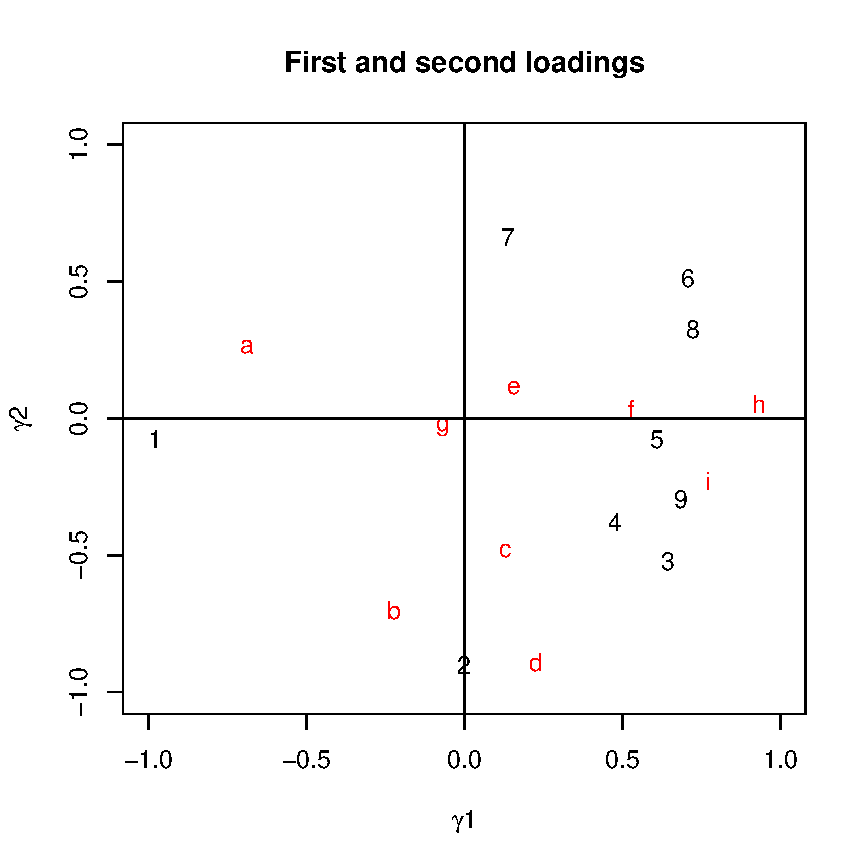
\includegraphics[width = 0.5\textwidth]{images/farotation}
\caption{Plot overlaying the co-ordinates of factor loadings 1 and 2 before and after rotation optimised by the varimax criterion}
\label{farotation}
\end{center}
\end{figure}

Although is is more difficult to see what is going on with $q=4$, we can see for example that the eighth variable (Social and Personal Services) has in increased loading in terms of $\gamma_{18}$, and a much decreased loading in terms of the second factor ($\gamma_{28}$ is virtually zero.   Thus we may feel that we have achieved some simplification of our factor structure.

\section{Factor scoring}

Finally, there are occasions where we may wish to estimate values for $\boldsymbol{\phi}_{i}$ for a given individual $i$.   These values are referred to as the scores, the process of estimating them, which has to be carried out after $\boldsymbol{\Gamma}$ and $\boldsymbol{\psi}$ have been estimated is therefore referred to as scoring.

Two methods are available in R for scoring, Thomson and Bartlett's.   The default is that no scoring takes place (it requires a data matrix).   By including \texttt{scores = "Bartlett")} or \texttt{scores = "regression"} these estimates are obtained.

\cite{Bartlett:1937,Bartlett:1938} propsed a method based upon weighted least squares.

Once we have estimates


\begin{eqnarray*}
x_{1} - \bar{x}_{1}  &=& \sum_{k=1}^{q} \hat{\gamma}_{1k} \phi_{1}  + \zeta_{1}\\
x_{2} - \bar{x}_{2} &=&  \sum_{k=1}^{q} \hat{\gamma}_{2k} \phi_{2}  + \zeta_{2}\\
&\vdots&\\
x_{p} - \bar{x}_{p} &=& \sum_{k=1}^{q} \hat{\gamma}_{pk} \phi_{p}  + \zeta_{p}
\end{eqnarray*}

we need to estimate $\phi_{j}$ for $j=1, \ldots, q$, however as $var(\zeta_{j}) = \psi_{j} $ are not equal he argued that weighted least squares was the most appropriate technique.

The weighted least squares estimates thus obtained are:

\begin{equation}
\boldsymbol{\hat{\phi}}_{i} = (\boldsymbol{\Gamma}^{T} \boldsymbol{\Psi}^{-1} \boldsymbol{\Gamma})\boldsymbol{\Gamma}^{T} \boldsymbol{\Psi}(\boldsymbol{x}_{i} - \boldsymbol{\bar{x}})
\end{equation}

\cite{Thomson:1951} is based on assuming that both $\boldsymbol{\phi}$ and $\boldsymbol{\zeta}$ are multivariate normal, thus a concatenation of the manifest ($\boldsymbol{x}$) and latent ( $\boldsymbol{\phi}$) variables $\boldsymbol{y}^{T} = (\boldsymbol{\phi}^{T}, \boldsymbol{x}^{T})$ will also be normal with dispersion matrix:

\begin{displaymath}
var(\boldsymbol{y}) = \left( \begin{array}{cc} \boldsymbol{I} & \boldsymbol{\Gamma}^{T} \\
\boldsymbol{\Gamma} & \boldsymbol{\Gamma} \boldsymbol{\Gamma}^{T} + \boldsymbol{\psi} \end{array} \right)
\end{displaymath}


The mean of $\boldsymbol{\phi}$ is zero by definition, therefore:

\begin{displaymath}
E(\boldsymbol{z} | \boldsymbol{x}_{0}) =  \boldsymbol{\Gamma}^{T}(\boldsymbol{\Gamma})\boldsymbol{\Gamma}^{T} + \boldsymbol{\Psi})^{-1}(\boldsymbol{x}_{o} - \boldsymbol{\mu})
\end{displaymath}

which gives the estimate for the scores as:

\begin{equation}
\boldsymbol{z} =  \boldsymbol{\hat{\Gamma}}^{T}(\boldsymbol{\hat{\Gamma}})\boldsymbol{\hat{\Gamma}}^{T} + \boldsymbol{\hat{\psi}})^{-1}(\boldsymbol{x}_{i} - \boldsymbol{\hat{mu}})
\end{equation}

It might be clear that factor scoring takes no account of uncertainty in the estimates of $\boldsymbol{\hat{\Gamma}}$ and $ \boldsymbol{\hat{\psi}}$, this is one area where Bayesian methods are coming to the fore \citep{Aitkin+Aitkin:2005}


%As stated, Factor Analysis is very common in application areas such as Psychometrics.   The canonical example is an analysis of intelligence testing.  We will use an example from Smith, G. A. and Stanley G. (1983) ``Clocking g: relating intelligence and measures of timed performance''. Intelligence, 7, 353-368 (presented in Bartholomew, 1990).   If we load up the \texttt{ability.cov} object we have a covariance matrix arising from six tests given to 112 individuals.   The six tests are general: a non-verbal measure of general intelligence using Cattell's culture-fair test, picture: a picture-completion test, blocks: block design, maze: mazes, reading: reading comprehension and finally vocab: vocabulary.   The underlying theory is that there exists some kind of ``general intelligence'' ($g$); the more $g$ an individual has the higher they will tend to score in all of the six tests. 

%The following code will fit a Factor Analysis model by maximum likelihood to this covariance matrix; a set of calls to \texttt{update} will increase the number of latent variables to two, and will also fit different rotations.   Part of the rationale for carrying out the rotations is to produce more readily interpreted factors.   In the case of promax, the rotation yields a number of loadings which are essentially zero.

%Bartholomew gives both covariance and correlation matrices, but these are inconsistent. Neither are in the original paper. 

%Barthlomew, D. J. (1987) Latent Variable Analysis and Factor Analysis. Griffin. 
%Barthlomew, D. J. and Knott, M. (1990) Latent Variable Analysis and Factor Analysis. Second Edition, Arnold. 


%\singlespacing
%\begin{verbatim}
%> ability.cov ## have a look at the covariance matrix
%> ?ability.cov ## get some details on the ``data''
%> ability.FA <- factanal(factors = 1, covmat=ability.cov, rotation = "none")
%> ability.FA ## have a look at the first model
%> update(ability.FA, factors=2) ## what about two latent variables
%> update(ability.FA, factors=2, rotation="varimax")
%> update(ability.FA, factors=2, rotation="promax")
%\end{verbatim}
%\onehalfspacing

%\textit{How do you interpret the various models?}   Most of our work in factor analysis will be considered with rotation and reificaton (interpreting the hidden variables).

%%% Local Variables: ***
%%% mode:latex ***
%%% TeX-master: "../book.tex"  ***
%%% End: ***